\documentclass{standalone}
\usepackage{tikz}
\usetikzlibrary{arrows,decorations.markings,decorations.pathreplacing,calc,positioning}

\ifdefined\argstart
\fi

\ifdefined\argiterlabel
   \def\drawiterlabel{}
\fi

\ifdefined\argcandidatea
   \def\drawiterlabel{}
   \def\drawcandidatea{}
\fi

\ifdefined\argcandidateadelta
   \def\drawiterlabel{}
   \def\drawcandidatea{}
   \def\drawcandidateadelta{}
\fi

\ifdefined\argcandidateaeval
   \def\drawiterlabel{}
   \def\drawcandidatea{}
   \def\drawcandidateadelta{}
   \def\drawcandidateaeval{}
\fi

\ifdefined\argcandidateb
   \def\drawiterlabel{}
   \def\drawcandidatea{}
   \def\drawcandidateb{}
\fi

\ifdefined\argcandidatebdelta
   \def\drawiterlabel{}
   \def\drawcandidatea{}
   \def\drawcandidateb{}
   \def\drawcandidatebdelta{}
\fi

\ifdefined\argcandidatebeval
   \def\drawiterlabel{}
   \def\drawcandidatea{}
   \def\drawcandidateb{}
   \def\drawcandidatebdelta{}
   \def\drawcandidatebeval{}
\fi

\ifdefined\argprefinal
   \def\drawiterlabel{}
   \def\drawcandidatea{}
   \def\drawcandidateb{}
   \def\drawcandidatebeval{}
   \def\drawothercandidates{}
\fi

\ifdefined\argfinal
   \def\drawiterlabel{}
   \def\drawcandidatea{}
   \def\drawcandidateb{}
   \def\drawcandidatebeval{}
   \def\drawothercandidates{}
   \def\drawfinal{}
\fi

\begin{document}%
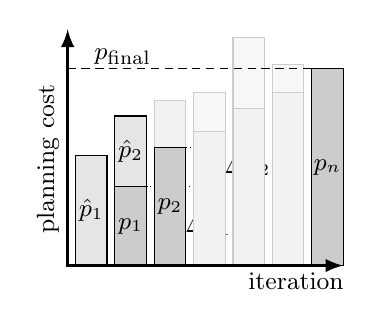
\begin{tikzpicture}[font=\small]

%\draw[black!5] (-0.1,-0.1) rectangle (3.6,3.6);
%\draw[step=0.5cm,black!20,very thin] (0,0) grid (3.5,3.5);

% some bars

\ifdefined\drawcandidatea
   % col1
   \draw[fill=black!10] (0.1,0) rectangle node[anchor=center]{$\hat{p}_1$} (0.5,1.4);
\fi


\ifdefined\drawcandidateadelta
   %\draw[densely dotted] (1.0,1.0) -- (1.8,1.0);
   \draw[densely dotted] (1.0,1.0) -- (1.3,1.0);
   \draw [decorate,decoration={brace,amplitude=3pt,mirror},xshift=0pt,yshift=0pt]
   (1.3,0.0) -- (1.3,1.0) node[anchor=west] [black,midway,xshift=2pt] 
   {$\Delta p_1$};
\fi

\ifdefined\drawcandidatebdelta
   \draw[densely dotted] (1.0,1.0) -- (1.8,1.0);
   \draw[densely dotted] (1.5,1.5) -- (1.8,1.5);
   \draw [decorate,decoration={brace,amplitude=3pt,mirror},xshift=0pt,yshift=0pt]
   (1.8,1.0) -- (1.8,1.5) node[anchor=west] [black,midway,xshift=2pt] 
   {$\Delta p_2$};
\fi

% col 2
\ifdefined\drawcandidateaeval
   \draw[fill=black!20] (0.6,0.0) rectangle node[anchor=center]{$p_1$} (1.0,1.0);
\fi

\ifdefined\drawcandidateb
   % col1
   \draw[fill=black!20] (0.6,0.0) rectangle node[anchor=center]{$p_1$} (1.0,1.0);

   \draw[fill=black!10] (0.6,1.0) rectangle node[anchor=center]{$\hat{p}_2$} (1.0,1.9);
\fi

\ifdefined\drawothercandidates
   % col 3
   \draw[black!20,fill=black!05] (1.1,1.5) rectangle node[anchor=center]{} (1.5,2.1);

   % col 4
   \draw[black!20,fill=black!05] (1.6,0.0) rectangle node[anchor=center]{}   (2.0,1.7);
   \draw[black!20,fill=black!03] (1.6,1.7) rectangle node[anchor=center]{} (2.0,2.2);

   % col 5
   \draw[black!20,fill=black!05] (2.1,0.0) rectangle node[anchor=center]{}   (2.5,2.0);
   \draw[black!20,fill=black!03] (2.1,2.0) rectangle node[anchor=center]{} (2.5,2.9);

   % col 6
   \draw[black!20,fill=black!05] (2.6,0.0) rectangle node[anchor=center]{}   (3.0,2.2);
   \draw[black!20,fill=black!03] (2.6,2.2) rectangle node[anchor=center]{} (3.0,2.55);

   % col 7
   \draw[black,fill=black!20] (3.1,0.0) rectangle node[black,anchor=center]{$p_n$}   (3.5,2.5);
\fi

% col 3
\ifdefined\drawcandidatebeval
   \draw[fill=black!20] (1.1,0.0) rectangle node[anchor=center]{$p_2$}   (1.5,1.5);
\fi

\ifdefined\drawfinal

   \draw[densely dashed] (0,2.5) -- (3.5,2.5);

   \node at (0.7,2.65) {$p_{\mbox{\scriptsize final}}$};

\fi

% axes
\draw[black,very thick,latex-latex] (0,3.0) -- (0,0) -- (3.5,0);
\node[rotate=90] at (-0.25,1.35) {planning cost};

\ifdefined\drawiterlabel
   \node at (2.9,-0.2) {iteration};
\fi



\end{tikzpicture}
\end{document}
